\documentclass[a4paper,11pt]{article}
\pagestyle{headings}

\usepackage[utf8]{inputenc}
\usepackage[french]{babel}
\usepackage{graphicx}
\usepackage{float}
\usepackage{fullpage}
\usepackage{diagbox}
\usepackage{enumitem}
\usepackage[T1]{fontenc}
\graphicspath{{images/}}

\title{Reconnaissance de formes et apprentissage automatique Projet 1}
\author{Auriane Reverdell, Felix Hähnlein, Nicolas Violette, Romain Duléry}
\date{\today}

\setlength{\oddsidemargin}{0.2cm}
\setlength{\evensidemargin}{-0.7cm}
\setlength{\parindent}{30pt}
\setlength{\textwidth}{15cm}
\setlength{\textheight}{24cm}
\setlength{\topmargin}{-.5in}
\setlength{\parskip}{1ex}

\begin{document}

\maketitle
\vspace{1cm}

\section{Résumé du travail réalisé}

\section{Analyse des résultats expérimentaux}

    \subsection{Phase d'apprentissage}

	\subsubsection{Travail réalisé}

	\subsubsection{Analyse de l'influence des paramètres}

    \subsection{Détection faciale}

	\subsubsection{Détection de visage sans post-traitement}

	\subsubsection{Détection de visage avec post-traitement}

	\subsubsection{Évaluation des détections de visages}

\section{Conclusion}

\section{Notes Auriane pour qu'elle s'en rappelle}

    %TODO : faire une vraie analyse sur les paramètres

\section{Analyse qualitative des détections}
    
    \subsection{Orientation du visage}
	
	Dans l'image suivante (figure \ref{fig:visage_or1}), l'orientation du visage varie
	progressivement, cela nous montre exactement l'orientation à partir de laquelle la
	reconnaissance ne marche plus. Nous remarquons ici que la détection dépend de la présence
	des deux yeux, dès que l'un d'eux n'est plus visible ou occulté, la détection de fonctionne
	plus.

	\begin{figure}[H]
	    \begin{center}
		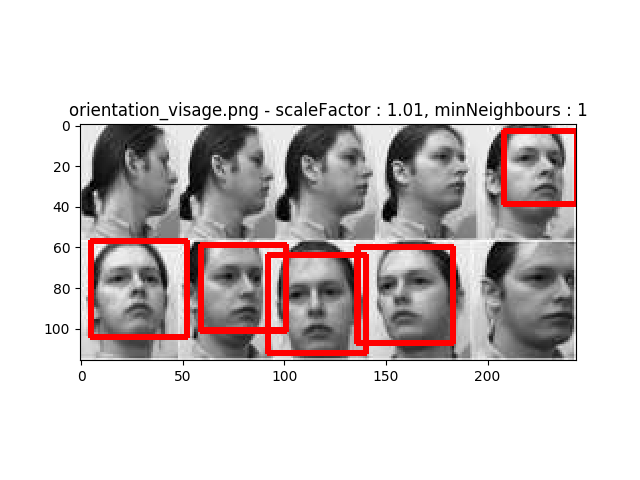
\includegraphics[scale = 0.6]{images/orientation_visage_1,01_1.png}
		\caption{Variation de l'orientation du visage - min neighbours = 1}
		\label{fig:visage_or1}
	    \end{center}
	\end{figure}

	Si l'on augmente \textit{minneighbours}, rien ne change jusqu'à 3 (figure
	\ref{fig:visage_or2}) puis le nombre de reconnaissance diminue.

	\begin{figure}[H]
	    \begin{center}
		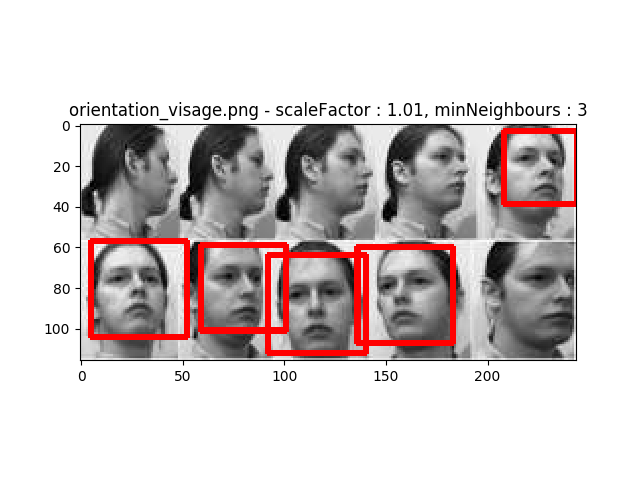
\includegraphics[scale = 0.6]{images/orientation_visage_1,01_3.png}
		\caption{Variation de l'orientation du visage - min neighbours = 3}
		\label{fig:visage_or2}
	    \end{center}
	\end{figure}

    \subsection{Expressions du visage}

	\begin{figure}[H]
	    \begin{center}
		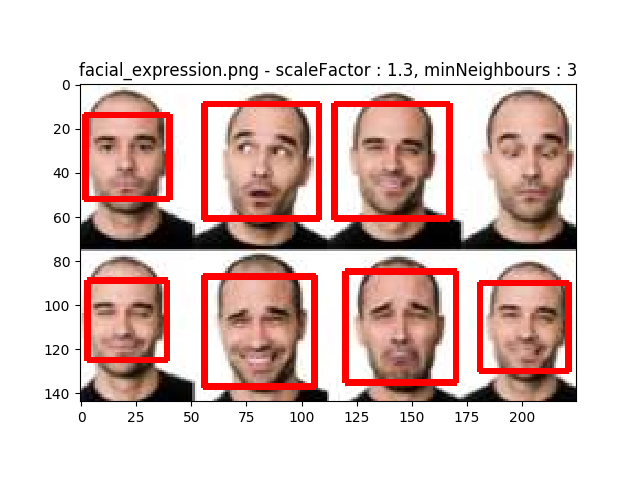
\includegraphics[scale = 0.6]{images/facial_expression_1,3_3.png}
		\caption{Changement d'expressions du visage}
		\label{fig:visage_exp}
	    \end{center}
	\end{figure}

    
    \subsection{Singes}

	Le singe est détecté lorsque le	\textit{scaleFactor} et le \textit{minNeighbours} sont
	relativement bas \ref{fig:singe}, dès que l'on augmente un peu l'un d'eux, la reconnaissance
	ne se fait plus.

	\begin{figure}[H]
	    \begin{center}
		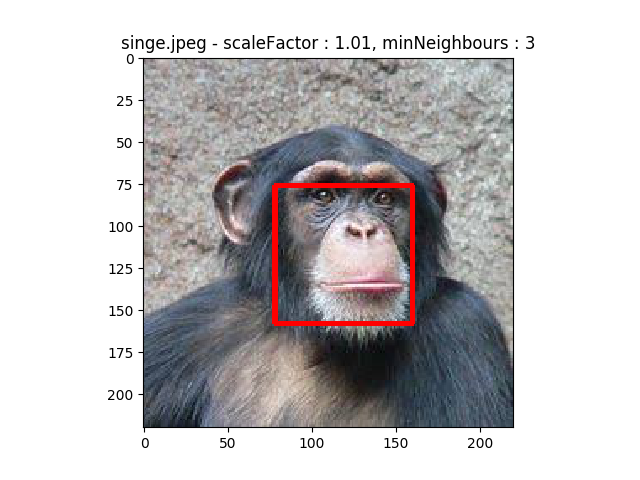
\includegraphics[scale = 0.6]{images/singe_1,01_3.png}
		\caption{Reconnaissance d'un singe}
		\label{fig:singe}
	    \end{center}
	\end{figure}

	Si l'on prend des paramètres identiques pour la reconnaissance du gorille (cela nous semble
	faisable car il y a une importante zone d'ombre au niveau des yeux du gorille), la
	reconnaissance ne marche pas, il faut augmenter le \textit{scaleFactor} à 1.021 pour qu'on
	ait des détections (cf figure \ref{fig:singe2}).

	\begin{figure}[H]
	    \begin{center}
		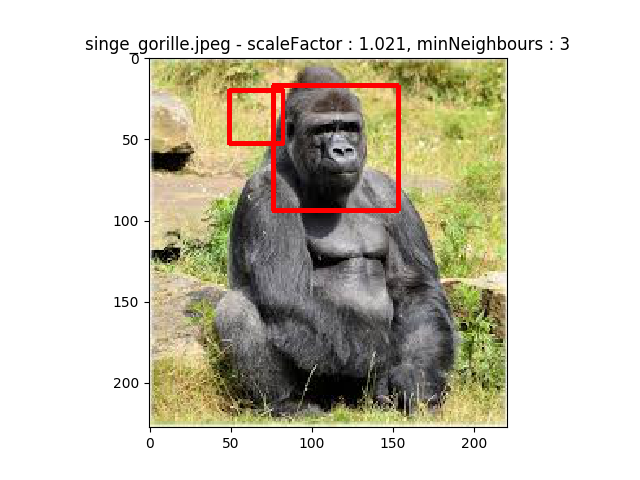
\includegraphics[scale = 0.6]{images/singe_gorille_1,021_3.png}
		\caption{Reconnaissance d'un gorille - scaleFactor = 1.021}
		\label{fig:singe2}
	    \end{center}
	\end{figure}

    \subsection{Occultations}

	\subsubsection{Oeil de pirate}

	    \begin{figure}[H]
	        \begin{center}
	    	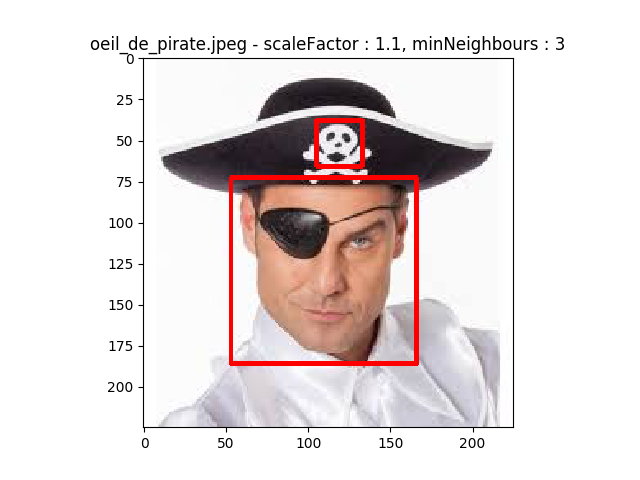
\includegraphics[scale = 0.6]{images/oeil_de_pirate_1,1_3.png}
	    	\caption{Reconnaissance d'un visage occulté}
	    	\label{fig:pirate}
	        \end{center}
	    \end{figure}

	\subsubsection{Lunettes de soleil}

	    Sur cette image le visage est orienté, la détection opère tout de même. En effet les
	    lunettes se positionnent à l'endroit des yeux, ce qui trompe le \textit{feature}
	    utilisé.

	    \begin{figure}[H]
	        \begin{center}
	    	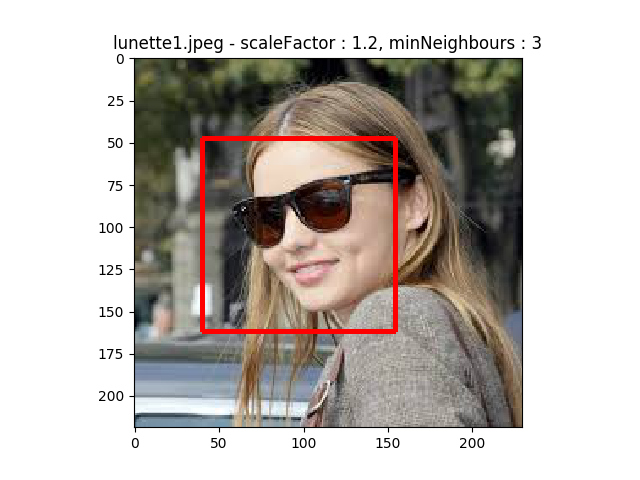
\includegraphics[scale = 0.6]{images/lunette1_1,2_3.png}
	    	\caption{Reconnaissance d'un visage occulté par des lunettes de soleil}
	    	\label{fig:lunette}
	        \end{center}
	    \end{figure}

\end{document}
